\documentclass{standalone}
\usepackage{tikz}
\usepackage{ctex,siunitx}
\usepackage{tkz-euclide}
\usepackage{amsmath}
\usetikzlibrary{patterns, calc}
\usetikzlibrary {decorations.pathmorphing, decorations.pathreplacing, decorations.shapes,}
\begin{document}
\small
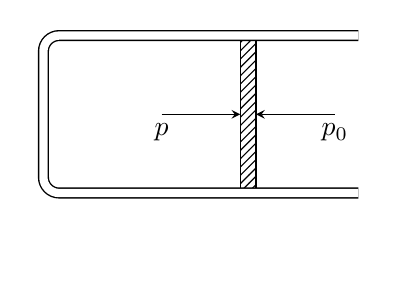
\begin{tikzpicture}[>=stealth,scale=1.0]
  \useasboundingbox(-0.2,0.1)rectangle(4.2,-3);
  \draw [pattern=north east lines](2.5,-2) rectangle (2.7,0);	
  \draw[->](1.5,-1) node [below]{$p$}--(2.5,-1);
  \draw[->](3.7,-1)node [below]{$p_0$}--(2.7,-1);
  \pgfsetlinewidth{4pt}
  \pgfsetinnerlinewidth{3pt}
  \draw [rounded corners=0.2cm](4,0)--(0,0)--(0,-2)--(4,-2);
\end{tikzpicture}
\end{document}